\documentclass[11pt]{scrreprt}
\usepackage{geometry}
\usepackage{graphicx, xcolor}
\usepackage{amsmath, amsfonts, amssymb, amsthm, mathtools, bm}
\usepackage{hyperref}
\usepackage[nameinlink]{cleveref}
\usepackage[all]{hypcap} % Links hyperref to object top and not caption
\usepackage[inline]{enumitem}
\usepackage{marginnote}
\usepackage[bottom]{footmisc}

\geometry{ margin=3cm, lmargin=2cm, rmargin=4cm, marginparwidth=3cm }
\hypersetup{ colorlinks, citecolor=black, filecolor=black, linkcolor=black, urlcolor=black, linktoc=all }

\NewDocumentEnvironment{descriptionlist}{}{%
  \begin{description}[labelindent=1em]
}{
  \end{description}%
}
\setlength{\parindent}{0pt}
\renewcommand*{\marginfont}{\color{gray}\footnotesize}

\theoremstyle{definition}
\newtheorem{theorem}{Theorem}[section]
\newtheorem*{example}{Example}
\theoremstyle{definition}
\newtheorem*{definition}{Def}

\newcommand{\ubar}[1]{\text{\b{$#1$}}}
\renewcommand{\vec}[1]{{\bm{#1}}}
\newcommand{\nullvec}[0]{\bar{\vec{0}}}
\newcommand{\matr}[1]{{\bm{#1}}}



\title{Fundamentals of Artificial Intelligence and Knowledge Representation}
\date{2023 -- 2024}

\begin{document}
\newgeometry{margin=3cm}
    \makeatletter
    \begin{titlepage}
        \centering
        \vspace*{\fill}
        \huge
        \textbf{\@title}
        \vspace*{\fill}

        \Large
        Academic Year \@date\\
        Alma Mater Studiorum $\cdot$ University of Bologna
        \vspace*{1cm}
    \end{titlepage}
    \makeatother
    \pagenumbering{roman}
    \tableofcontents
\restoregeometry
    \newpage
    \pagenumbering{arabic}

    \lohead{\color{gray} Not required for the exam}
\lehead{\color{gray} Not required for the exam}
\chapter{Introduction}


\section{AI systems classification}

\subsection{Intelligence classification}
Intelligence is defined as the ability to perceive or infer information and to retain the knowledge for future use.

\begin{description}
    \item[Weak AI] \marginnote{Weak AI}
        aims to build a system that acts as an intelligent system. 
    
        \item[Strong AI] \marginnote{Strong AI}
        aims to build a system that is actually intelligent. 
\end{description}


\subsection{Capability classification}
\begin{description}
    \item[General AI] \marginnote{General AI}
        systems able to solve any generalized task. 
    
        \item[Narrow AI] \marginnote{Narrow AI}
        systems able to solve a particular task. 
\end{description}


\subsection{AI approaches}
\begin{description}
    \item[Symbolic AI (top-down)] \marginnote{Symbolic AI}
        Symbolic representation of knowledge, understandable by humans.

    \item[Connectionist approach (bottom-up)] \marginnote{Connectionist approach}
        Neural networks. Knowledge is encoded and not understandable by humans.
\end{description}



\section{Symbolic AI}
\begin{description}
    \item[Deductive reasoning] \marginnote{Deductive reasoning}
        Conclude something given some premises (general to specific). 
        It is unable to produce new knowledge.
        \begin{example}
            "All men are mortal" and "Socrates is a man" $\rightarrow$ "Socrates is mortal"
        \end{example}
    
    \item[Inductive reasoning] \marginnote{Inductive reasoning}
        A conclusion is derived from an observation (specific to general).
        Produces new knowledge, but correctness is not guaranteed.
        \begin{example}
            "Several birds fly" $\rightarrow$ "All birds fly"
        \end{example}

    \item[Abduction reasoning] \marginnote{Abduction reasoning}
        An explanation of the conclusion is found from known premises.
        Differently from inductive reasoning, it does not search for a general rule.
        Produces new knowledge, but correctness is not guaranteed.
        \begin{example}
            "Socrates is dead" (conclusion) and "All men are mortal" (knowledge) $\rightarrow$ "Socrates is a man"
        \end{example}
    
    \item[Reasoning by analogy] \marginnote{Reasoning by analogy}
        Principle of similarity (e.g. k-nearest-neighbor algorithm).
        \begin{example}
            "Socrates loves philosophy" and Socrates resembles John $\rightarrow$ "John loves philosophy"
        \end{example}

    \item[Constraint reasoning and optimization] \marginnote{Constraint reasoning}
        Constraints, probability, statistics.
\end{description}


\section{Machine learning}

\subsection{Training approach}
\begin{description}
    \item[Supervised learning] \marginnote{Supervised learning}
        Trained on labeled data (ground truth is known).\\
        Suitable for classification and regression tasks.

    \item[Unsupervised learning] \marginnote{Unsupervised learning}
        Trained on unlabeled data (the system makes its own discoveries).\\
        Suitable for clustering and data mining.

    \item[Semi-supervised learning] \marginnote{Semi-supervised learning}
        The system is first trained to synthesize data in an unsupervised manner,
        followed by a supervised phase.

    \item[Reinforcement learning] \marginnote{Reinforcement learning}
        An agent learns by simulating actions in an environment with rewards and punishments depending on its choices.
\end{description}


\subsection{Tasks}
\begin{description}
    \item[Classification] \marginnote{Classification}
        Supervised task that, given the input variables $X$ and the output (discrete) categories $Y$,
        aims to approximate a mapping function $f: X \rightarrow Y$.

    \item[Regression] \marginnote{Regression}
        Supervised task that, given the input variables $X$ and the output (continuous) variables $Y$,
        aims to approximate a mapping function $f: X \rightarrow Y$.

    \item[Clustering] \marginnote{Clustering}
        Unsupervised task that aims to organize objects into groups.
\end{description}


\subsection{Neural networks}
\marginnote{Perceptron}
A neuron (\textbf{perceptron}) computes a weighted sum of its inputs and 
passes the result to an activation function to produce the output.
\begin{figure}[h]
    \centering
    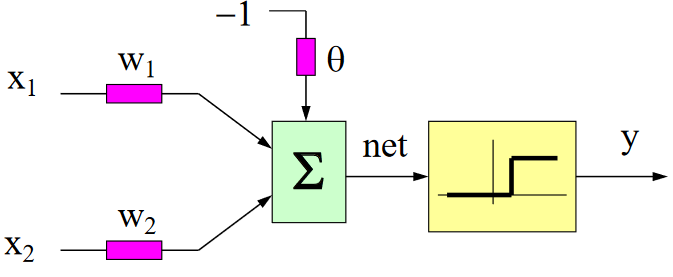
\includegraphics[width=0.40\textwidth]{img/neuron.png}
    \caption{Representation of an artificial neuron}
\end{figure}

\marginnote{Feed-forward neural network}
A \textbf{feed-forward neural network} is composed of multiple layers of neurons, each connected to the next one.
The first layer is the input layer, while the last is the output layer.
Intermediate layers are hidden layers.

The expressivity of a neural network increases when more neurons are used:
\begin{descriptionlist}
    \item[Single perceptron] 
        Able to compute a linear separation.
        \begin{figure}[h]
            \centering
            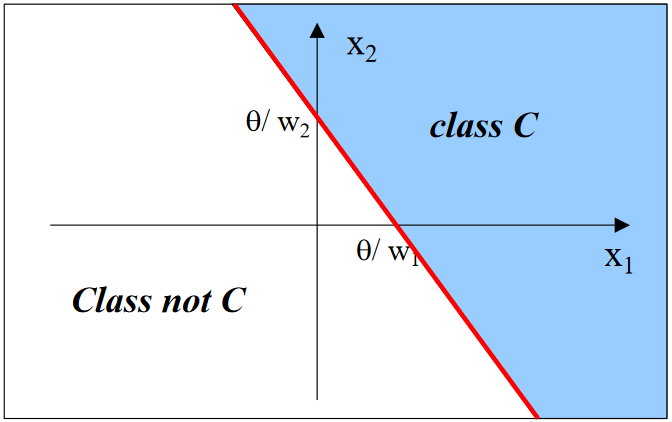
\includegraphics[width=0.25\textwidth]{img/1perceptron.png}
            \caption{Separation performed by one perceptron}
        \end{figure}
    \item[Three-layer network] 
        Able to separate a convex region ($n_\text{edges} \leq n_\text{hidden neurons}$)
        \begin{figure}[h]
            \centering
            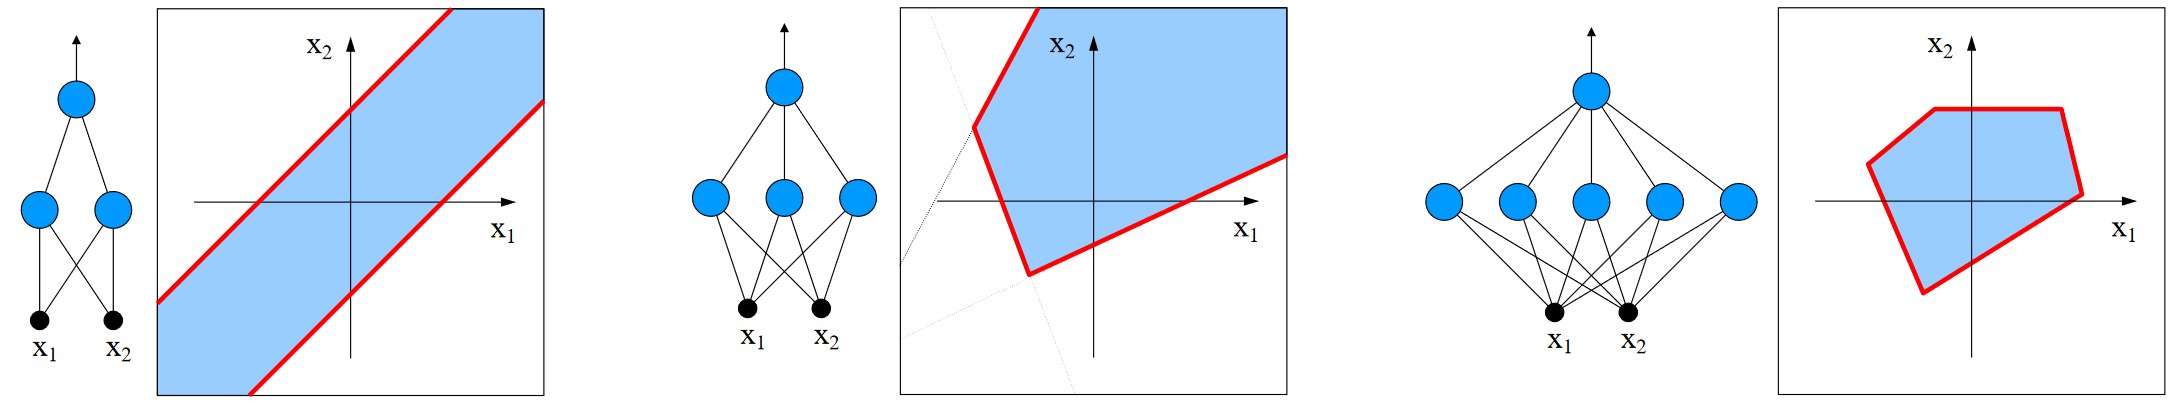
\includegraphics[width=0.90\textwidth]{img/3layer.png}
            \caption{Separation performed by a three-layer network}
        \end{figure}
    \item[Four-layer network] 
        Able to separate regions of arbitrary shape.
        \begin{figure}[h]
            \centering
            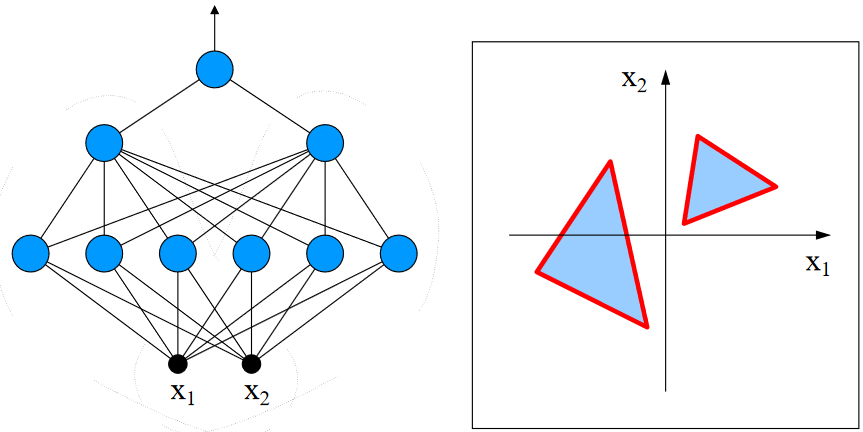
\includegraphics[width=0.40\textwidth]{img/4layer.png}
            \caption{Separation performed by a four-layer network}
        \end{figure}
\end{descriptionlist}

\begin{theorem}[Universal approximation theorem] \marginnote{Universal approximation theorem}
    A feed-forward network with one hidden layer and a finite number of neurons is
    able to approximate any continuous function with desired accuracy.
\end{theorem}

\begin{description}
    \item[Deep learning] \marginnote{Deep learning}
        Neural network with a large number of layers and neurons.
        The learning process is hierarchical: the network exploits simple features in the first layers and
        synthesizes more complex concepts while advancing through the layers.
\end{description}



\section{Automated planning}
Given an initial state, a set of actions and a goal, 
\textbf{automated planning} aims to find a partially or totally ordered sequence of actions to achieve a goal. \marginnote{Automated planning}

An \textbf{automated planner} is an agent that operates in a given domain described by:
\begin{itemize}
    \item Representation of the initial state
    \item Representation of a goal
    \item Formal description of the possible actions (preconditions and effects)
\end{itemize}



\section{Swarm intelligence}
\marginnote{Swarm intelligence}
Decentralized and self-organized systems that result in emergent behaviors. 



\section{Decision support systems}

\begin{description}
    \item[Knowledge based system] \marginnote{Knowledge based system}
        Use knowledge (and data) to support human decisions.
        Bottlenecked by knowledge acquisition.
\end{description}

Different levels of decision support exist:
\begin{descriptionlist}
    \item[Descriptive analytics] \marginnote{Descriptive analytics}
        Data are used to describe the system (e.g. dashboards, reports, \dots).
        Human intervention is required.
            
    \item[Diagnostic analytics] \marginnote{Diagnostic analytics}
        Data are used to understand causes (e.g. fault diagnosis)
        Decisions are made by humans.

    \item[Predictive analytics] \marginnote{Predictive analytics}
        Data are used to predict future evolutions of the system.
        Uses machine learning models or simulators (digital twins)

    \item[Prescriptive analytics] \marginnote{Prescriptive analytics}
        Make decisions by finding the preferred scenario.
        Uses optimization systems, combinatorial solvers or logical solvers.
\end{descriptionlist}


\newpage
\lohead{}
\lehead{}



\end{document}